\documentclass[11pt]{article}
\usepackage{graphicx}
\usepackage{times}
\textwidth 6.5in
\topmargin 0.0in
\textheight 8.5in
\headheight 0in
\headsep 0in
\oddsidemargin 0in

\title{XORP Router Manager Process (rtrmgr) \\
\vspace{1ex}
Version 0.1}
\author{ XORP Project					\\
	 International Computer Science Institute	\\
	 Berkeley, CA 94704, USA			\\
	 {\it feedback@xorp.org}
}
\date{December 11, 2002}

%\twocolumn
\begin{document}
\maketitle                            
\section{Introduction}
This document provides a high-level technical overview of the Router
Manager (rtrmgr) code structure, intended to aid anyone needing to
understand or modify the software.   It is not a user manual.

The XORP software base consists of a number of routing protocols (BGP,
OSPF, PIM-SM, etc), a Routing Information Base (RIB) process, a
Forwarding Engine Abstraction (FEA) process, and a forwarding path.
Other management, monitoring or application processes may also
supplement this set.  Figure \ref{overview} illustrates these
processes and their principle communication channels.

\begin{figure}[htb]
\centerline{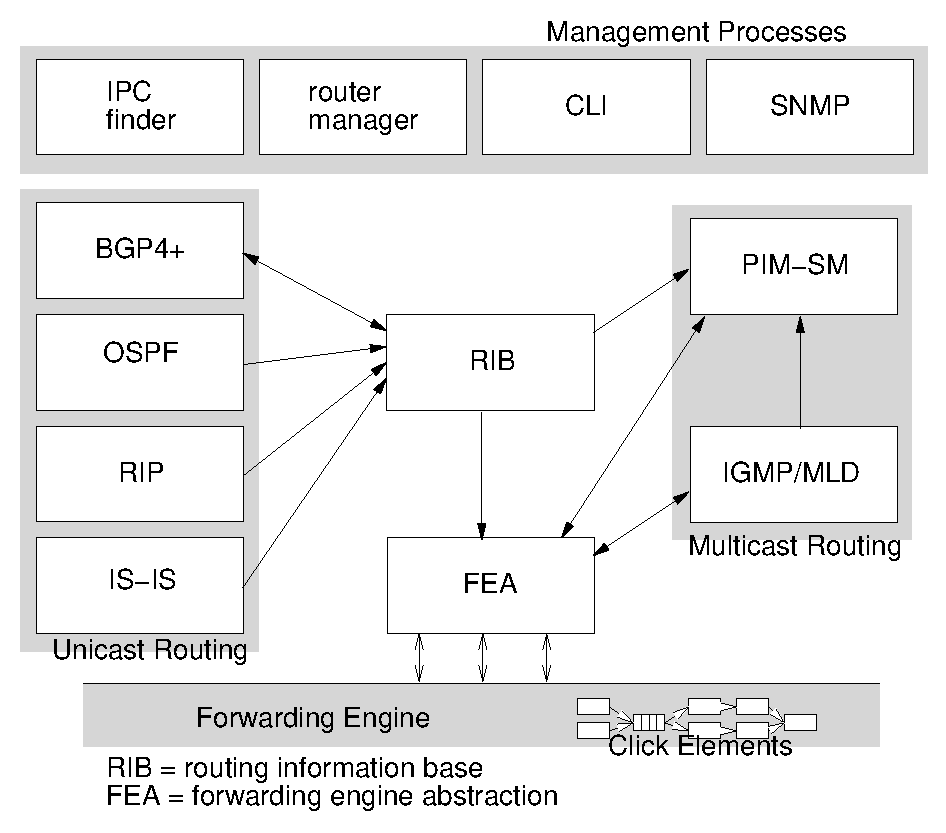
\includegraphics[width=0.6\textwidth]{figs/processes3}}
\vspace{.05in}
\caption{\label{overview}Overview of XORP processes}
\end{figure}

For research purposes, these processes may be started manually or from
scripts, so long as the dependencies between then are satisfied.  But
when using XORP in a more operational environment, the network manager
typically does not wish to see the software structure, but rather
would like to interact with the router {\it as a whole}.  Minimally, this
consists of a configuration file for router startup, and a command
line interface to interact with the router during operation.  The
rtrmgr process provides this unified view of the router.

The rtrmgr is normally the only process explicitly started at router
startup.  The rtrmgr process includes a built-in XRL finder, so no
external finder process is required.  The following sequence of
actions then occurs:
\begin{enumerate}
\item The rtrmgr reads all the template files in the router's template
directory.  Typically there is one template file per XORP process that
might be needed.  A template file describes the functionality that is
provided by the corresponding process in terms of all of the
configuration parameters that may be set.  It also describes the
dependencies that need to be satisfied before the process can be
started.  After reading the template files, the rtrmgr knows all the
configuration parameters currently supportable on this router, and it
stores this information in its \textit{template tree}.
\item
The rtrmgr next reads the contents of the XRL directory to discover
all the XRLs that are supported by the processes on this router.
These XRLs are then checked against the XRLs in the template tree.  As
it is normal for the XRLs in the XRL directory to be used to generate
stub code in the XORP processes, this forms the definitive version of
a particular XRL.  Checking against this version detects if a template
file has somehow become out of sync with the router's codebase.  Doing
this check at startup prevents subtle run time errors later.  The
rtrmgr will exit if a mismatch is discovered.
\item 
The rtrmgr then reads the router configuration file.  All the
configuration options in the config file must correspond to
configurable functionality as described by the template files.  As it
reads the config file, the rtrmgr stores the intended configuration in
its \textit{configuration tree}.  At this point, the nodes in the
configuration tree are annotated as \textit{not existing} - that is
this part of the configuration has not yet been communicated to the
process that will implement the functionality.
\item
The rtrmgr next traverses the configuration tree to discover the list
of processes that need to be started to provide the required
functionality.  Typically not all the available software on the router
will be needed for a specific configuration.
\item
The rtrmgr traverses the template tree again to discover an order for
starting the required processes that satisfies all their dependencies.
\item
The rtrmgr starts the first process in the list of processes to be
started.
\item
If no error occurs, the rtrmgr traverses the configuration tree to
build the list of XRLs that need to be called to configure the process
just started.  These XRLs are then called, one after another, with the
successful completion of one XRL triggering the calling of the next.
Some processes may require calling a transaction start XRL before
configuration, and a transaction complete XRL after configuration -
the rtrmgr can do this if required.
\item
If no error occurred during configuration, the next process is started,
and configured, and so forth, until all the required processes are
started and configured.
\item 
At this point, the router is up and running.  The rtrmgr will now
allow connections from the xorpsh process to allow interactive
operation.
\end{enumerate}
\newpage
\section{Template Files}
The router manager reads a directory of template files to discover the
configuration options that the router supports.  A fragment of such a
configuration file might look like:
\begin{verbatim}
protocols {
  ospf {
    router-id: ipv4;
    mospf: toggle = false;
    flood_rate: int;
    area @: ipv4 {
      stub: toggle = false;
      interface @: text {
        disable: toggle = false;
        hello-interval: uint = 30;
        dead-interval: uint = 95;
      }
    }
  }
}
\end{verbatim}
This defines a subset of the configuration options for OSPF.  The
configuration options form a tree, with three types of nodes:
\begin{itemize}
\item Structural nodes such as {\tt protocol} and {\tt ospf} that exist
merely to provide scope.
\item Named interior nodes such as ``{\tt area @}'' and ``{\tt interface @}'',
where there can be multiple instances of the node.  Here indicates
that a name is required; in the case of ``area @'' the fragment above
specifies that the name must be an IPv4 address.
\item Leaf nodes such as  {\tt flood\_rate} and
{\tt hello-interval}.  These nodes are also typed, and may optionally
specify a default value.  In the example above, {\tt hello-interval} is
of type {\tt uint} (unsigned 32 bit integer), and takes the default value of
30.
\end{itemize}
Thus the template tree created from this template file would look
like:
\begin{figure}[htb]
\centerline{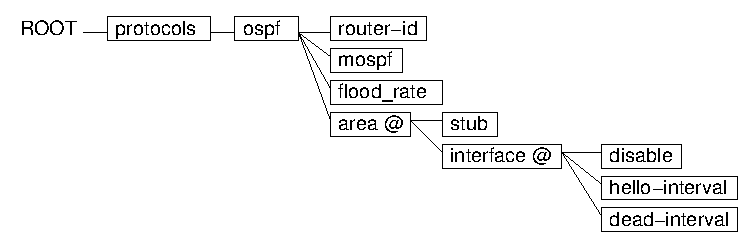
\includegraphics[width=0.7\textwidth]{figs/template}}
\vspace{.05in}
%\caption{\label{overview}Overview of XORP processes}
\end{figure}

The same node may occur multiple times in the template file.  This
might happen because the node can take more than one type (for
example, it might have an IPv4 or an IPv6 address), or it might happen
because the second definition adds information to the existing
definition.

In addition to specifying the configurable options, the template file
should also specify what the rtrmgr should do when an option is
modified.  These commands annotating the template file begin with a
``{\tt \%}''.  Thus the template file above might also contain the
following annotated version of the template tree:
\begin{verbatim}
protocols ospf {
  %modinfo: provides ospf;
  %modinfo: depends rib;
  %modinfo: path "../ospfd/xorp/ospfd";
  router-id {
    %set: xrl "ospf/ospf/0.1/set_router_id?id:u32=$(@)";
    %get: xrl "ospf/ospf/0.1/get_router_id->id:u32";
  }
  area @ {
    %create: xrl "ospf/ospf/0.1/add_or_configure_area?
                  area_id:u32=$(area.@)&is_stub:bool=$(@.stub)";
    %delete: xrl "ospf/ospf/0.1/delete_area?area_id:u32=$(area.@)";
  }
}
\end{verbatim}
The first three annotations apply to the ``protocols ospf'' node, and
specify the ``\%modinfo'' command, which provides information about
the module providing this functionality.  In this case they specify
that this functionality is provided by the module called {\tt ospf},
that this module depends on the module called {\tt rib}, and that the
software in {\tt ../ospfd/xorp/ospfd} is the software to run to
provide this module.

The ``{\tt protocols ospf router-id}'' node carries annotations to set
the value of the router ID in the ospf process, and to get the value
back.  The set command is:
\begin{verbatim}
    %set: xrl "ospf/ospf/0.1/set_router_id?id:u32=$(@)";
\end{verbatim}
This specifies that to set this value, the rtrmgr must call the
specified XRL.  In this case it specifies a variable expansion of the
variable {\tt \$(@)}.  All variables take the form {\tt \$(}...{\tt
)}.   

The variable {\tt \$(@)} means the value of the
current node, so if the router ID node in the configuration tree had
the value 1.2.3.4, then the XRL to call would be:
\begin{verbatim}
    ospf/ospf/0.1/set_router_id?id:u32=1.2.3.4
\end{verbatim}
The {\tt \%set} command only applies to leaf nodes.  

Internal nodes would typically use the {\tt \%create} command to
create a new instance of the node, as shown with the ``{\tt protocols ospf
area @}'' node.  In the example above, the {\tt \%create} command
involves two variable expansions: {\tt \$(area.@)} and {\tt
\$(@.stub)}.  The form {\tt \$(area.@)} means ``this area'', and so
in this case it is directly equivalent to {\tt \$(@)} meaning ``this node''.
The variable {\tt \$(@.stub)} means the value of the leaf node called
{\tt stub} that is a child node of ``this node''.

Thus the template tree specifies the following information:
\begin{itemize}
\item The nodes of the tree specify all the configuration options
possible on the router.
\item Some of the nodes are annotated with information to indicate
which software to run to provide the functionality rooted at that
node, and to indicate which other modules this software depends on
being running.
\item Most of the nodes are annotated with commands to be run when the
value of the node changes in the configuration tree, when a new
instance of the node is created or an instance of the node is deleted
in the configuration tree, or to get the current value of a node from
the running processes providing the functionality.
\end{itemize}
\subsection{Template Tree Node Types}
The following types are currently supported for template tree nodes:
\begin{description}
\item{\tt uint}\\
Unsigned 32 bit integer
\item{\tt int}\\
Signed 32 bit integer
\item{\tt bool}\\
Boolean - valid values are {\tt true} and {\tt false}.
\item{\tt toggle}\\
Similar to boolean, but requires a default value.  Display of the
config tree node is suppressed if the value is the default.
\item{\tt ipv4}\\
An IPv4 address in dotted decimal format.
\item{\tt ipv4\_prefix}\\ An IPv4 address and prefix length in the
conventional format.  E.g.: {\tt 1.2.3.4/24}.
\item{\tt ipv6}\\
An IPv6 address in the canonical colon-separated human-readable format.
\item{\tt ipv6\_prefix}\\
An IPv6 address and prefix in the conventional format. E.g.: {\tt
fe80::1/64}
\item{\tt macaddr}\\
An MAC address in the conventional colon-separated hex format.  E.g.:
{\tt 00:c0:4f:68:8c:58}
\end{description}
It is likely that additional types will be added in the future, as
they are found to be needed.

\subsection{Template Tree Commands}
This section provides a complete listing of all the template tree
commands that the rtrmgr supports.
\subsubsection{The {\tt \%modinfo} Command.}
The sub-commands to the {\tt \%modinfo} command are:
\begin{description}
\item {{\tt \%modinfo provides }{\it ModuleName}}  \\The {\tt provides} subcommand takes one additional
parameter, which gives the name of the module providing the
functionality rooted at this node.  
\item {{\tt \%modinfo depends }{\it list of modules}}  \\The {\tt depends} subcommand takes at least one additional
parameter, giving a list of the other modules that must
be running and configured before this module may be started.
\item {{\tt \%modinfo path }{\it ProgramPath}}  \\The {\tt path} subcommand takes one additional parameter giving the pathname of the software to be run
to provide this functionality.  The pathname may be absolute or
relative.
\item {{\tt \%modinfo startcommit }{\it XRL}}  \\The {\tt startcommit} subcommand takes one additional
parameter, and gives the XRL to call before performing
any change to the configuration of the module.
\item {{\tt \%modinfo endcommit }{\it XRL}}  \\The {\tt endcommit} subcommand takes one additional
parameter, and gives the XRL to call to complete any
change to the configuration of the module.  startcommit and
endcommit are optional.  They provide a way to make batch changes to a
module configuration as an atomic operation.
\end{description}
\subsubsection{The {\tt \%create} Command.}
{\tt \%create} is used to create a new instance of an interior node in
the configuration tree.  
\begin{itemize}
\item The first parameter indicates the form of
action to take to perform this action - typically it is {\tt xrl}
which indicates an XRL should be called.  
\item If the action is {\tt xrl}, then the second parameter gives the XRL to
call to create the new configuration tree instance of this template
tree node.
\end{itemize}

\subsubsection{The {\tt \%activate} Command.}
{\tt \%activate} is used to activate a new instance of an interior
node in the configuration tree.  It is typically paired with {\tt
\%create} - the {\tt \%create} command is executed before the relevant
configuration of the node's children has been performed, whereas {\tt
\%activate} is executed after the node's children have been
configured.  A particular interior node might have either {\tt
\%create}, {\tt \%activate} or both.
\begin{itemize}
\item The first parameter indicates the form of action to take to perform
this action - typically it is {\tt xrl} which indicates an XRL should
be called.
\item If the action is {\tt xrl}, then the second parameter gives the XRL to
call to activate the new configuration tree instance of this template
tree node
\end{itemize}

For example, if the template tree held the following:
\begin{tabbing}
\tt addr\=\tt ess \=\tt@: ipv4 \{\\
    \>\tt\%create: xrl {\it XRL1}\\
    \>\tt\%activate: xrl {\it XRL2}\\
    \>\tt netmask: ipv4 \{\\
        \>\>\tt\%set: xrl {\it XRL3}\\
    \>\tt\}\\
\tt\}
\end{tabbing}
Then when an instance of address and netmask are created and
configured, the execution order of the XRLs will be: {\it XRL1, XRL3, XRL2}.

\subsubsection{The {\tt \%list} Command.}
{\tt \%list} is called to obtain a list of all the configuration tree
instances of a particular template tree node.  For example, a
particular template tree node might represent the interfaces on a
router.  The configuration tree would then contain an instance of this
node for each interface currently configured.  The {\tt \%list}
command on this node would then return the list of interfaces.
\begin{itemize}
\item The first parameter indicates the form of action to take to perform
this action - typically it is {\tt xrl} which indicates an XRL should
be called.
\item If the action is {\tt xrl}, then the second parameter gives the XRL to
call to return the list.
\end{itemize}

\subsubsection{The {\tt \%delete} Command.}
{\tt \%delete} is called to delete a configuration tree node and all its
children.  A node that has a {\tt \%create} or {\tt \%activate}
command should also have a {\tt \%delete} command.
\begin{itemize}
\item The first parameter indicates the form of action to take to perform
this action - typically it is {\tt xrl} which indicates an XRL should
be called.
\item If the action is {\tt xrl}, then the second parameter gives the XRL to
call to delete the configuration tree instance of this template tree
node.
\end{itemize}

\subsubsection{The {\tt \%set} Command.}
{\tt \%set} is called to set the value of a leaf node in the
configuration tree.
\begin{itemize}
\item The first parameter indicates the form of action to take to perform
this action - typically it is {\tt xrl} which indicates an XRL should
be called.
\item If the action is {\tt xrl}, then the second parameter gives the XRL to
call to set the value of configuration tree instance of this template
tree node.
\end{itemize}
\subsubsection{The {\tt \%unset} Command.}
{\tt \%unset} is called to unset the value of a leaf node in the
configuration tree.  The value will return to its default value if a
default value is specified.
\begin{itemize}
\item The first parameter indicates the form of action to take to perform
this action - typically it is {\tt xrl} which indicates an XRL should
be called.
\item If the action is {\tt xrl}, then the second parameter gives the XRL to
call to unset the value of configuration tree instance of this template
tree node.
\end{itemize}
\subsubsection{The {\tt \%get} Command.}
{\tt \%get} is called to get the value of a leaf node in the
configuration tree.  Normally the rtrmgr will know the value if there
is no external means to change the value, but the {\tt \%get} command
provides a way for the rtrmgr to re-sync if the value has changed.
\begin{itemize}
\item The first parameter indicates the form of action to take to perform
this action - typically it is {\tt xrl} which indicates an XRL should
be called.
\item If the action is {\tt xrl}, then the second parameter gives the XRL to
call to get the value of configuration tree instance of this template
tree node.
\end{itemize}
\subsubsection{The {\tt \%allow} Command.}
The {\tt \%allow} command provides a way to restrict the value of
certain nodes to specific values.
\begin{itemize}
\item The first parameter gives the name of the variable to be restricted.
\item The remaining parameters are a list of possible allowed values for
this variable.
\end{itemize}
For example, a node might specify an address family, which is intended
to be one of ``inet'' or ``inet6''.  The type of the node is {\tt
text}, which would allow any value, so the allow command might allow
the rtrmgr to restrict the legal values without having to
communicate with the process providing this functionality.

A more subtle use might be to allow certain nodes to exist only if a
parent node was of a certain value.

For example:
\begin{verbatim}
      family @: text {
        %allow: $(@) "inet" "inet6";
        address @: ipv4 {
          %allow: $(family.@) "inet";
          broadcast: ipv4;
        }
        address @: ipv6 {
          %allow: $(family.@) "inet6";
        }
      }
\end{verbatim}
In this case, there are two different typed versions of the ``{\tt
address @}'' node, once for IPv4 and one for IPv6.  Only one of them has
a leaf node called {\tt broadcast}.  The allow command permits the
rtrmgr to do type-checking to ensure that only the permitted
combinations are allowed.
\newpage
\section{The Configuration File}
Whereas the template files inform the rtrmgr as the {\it possible}
configuration of the router, the configuration file provides the
specific startup configuration to be used by this specific router.
The syntax is similar to, but not the same as, that of template files -
the differences are intentional - template files are intended to be
written by software developers, whereas configuration files are
intended to be written by network managers.  Hence the syntax of
configuration files is simpler and more intuitive, but less powerful.
However, both specify the same sort of tree structure, and the nodes
in the configuration tree must correspond to the nodes in the template
tree.

An example fragment of a configuration file might be:
\begin{verbatim}
protocols {
  ospf {
    router-id: 1.2.3.4
    mospf
    area 1.2.3.27 {
      stub
      interface fxp1 {
        hello-interval: 10
      }
      interface fxp2
    }
  }
}
\end{verbatim}
Note that unlike in the template tree, semicolons are not needed in the
configuration tree, and that line-breaks are significant.

The example fragment of a configuration file above will construct the
following configuration tree from the template tree example given
earlier:
\begin{figure}[htb]
\centerline{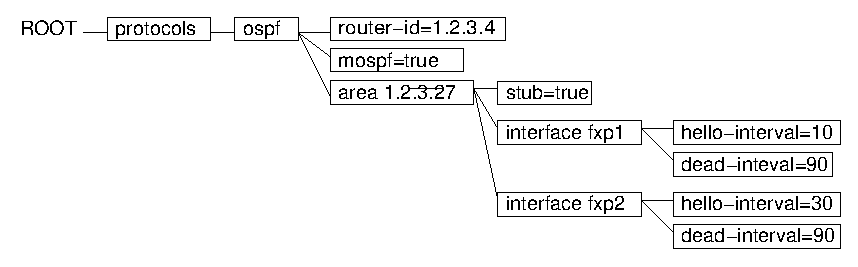
\includegraphics[width=0.7\textwidth]{figs/config}}
\vspace{.05in}
%\caption{\label{overview}Overview of XORP processes}
\end{figure}

Note that configuration tree nodes have been created for {\tt
dead-interval} and (in the case of fxp1) for {\tt hello-interval} even
though this was not mentioned in the configuration file.  This is
because the template tree contains a default value for this leaf node.
\newpage
\section{Command Line Interface: xorpsh}
The rtrmgr process is the core of a XORP router - it starts and stops
processes and keeps track of the configuration.  To do it's task, it
must run as root, whereas most other XORP processes don't need
privileged operation and so can be sandboxed.  This makes the rtrmgr
process the single most critical point from a security point of view.
Thus we would like the rtrmgr to be as simple as
possible\footnote{Unfortunately the router manager is not simple as we
would like.}, and to isolate it from possibly hostile input as far as
is reasonable.

For these reasons we do not build a command line interface directly
into the rtrmgr, but instead use an external process called {\tt
xorpsh} to interact with the user, while limiting the rtrmgr's
interaction with xorpsh to simple authentication mechanisms, and
exchanges of configuration tree data.  Thus the command line interface
architecture looks like:
\begin{figure}[htb]
\centerline{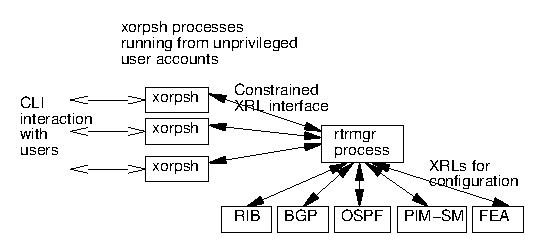
\includegraphics[width=0.7\textwidth]{figs/xorpsh}}
\vspace{.05in}
%\caption{\label{overview}Overview of XORP processes}
\end{figure}

The interface between the rtrmgr and a xorpsh instance consists of
XRLs that the xorpsh may call to query or configure rtrmgr, and a few
XRLs that the rtrmgr may asynchronously call to alert the xorpsh
process to certain events.  

The rtrmgr exports the following XRLs that may be called by xorpsh:
\begin{description}
\item{\tt register\_client} \\This XRL is used by a xorpsh instance to
register with the rtrmgr.  In response, the rtrmgr provides the name
of a file containing a nonce - the xorpsh must read this file and
return the contents to the rtrmgr to authenticate the user.
\item{\tt authenticate\_client} \\Xorpsh uses this to complete the
authentication process.
\item{\tt get\_running\_config} \\Xorpsh uses this to request the
current running configuration from the rtrmgr.  The response is text
in the same syntax as the rtrmgr configuration file that provides the
rtrmgr's view of the configuration.
\item{\tt enter\_config\_mode} \\A xorpsh process must be in
configuration mode to submit configuration changes to the rtrmgr.
This XRL requests that the rtrmgr allows the xorpsh to enter
configuration mode.  Not all users have permission to enter
configuration mode, and it is also possible that a request may be
refused because the configuration is locked.  
\item{\tt get\_config\_users} \\Xorpsh uses this to request the list of
users who are currently in configuration mode. 
\item{\tt apply\_config\_change} \\Xorpsh uses this to submit a request
to change the running configuration of the router to the rtrmgr.  The
change consists of a set of differences from the current running
configuration.
\item{\tt lock\_config} \\Xorpsh uses this to request an exclusive
lock on configuration changes.  Typically this is done just prior to
submitting a set of changes.
\item{\tt unlock\_config} \\Unlocks the rtrmgr configuration that was
locked by a previous call to {\tt lock\_config}.
\item{\tt lock\_node} \\Xorpsh uses this to request a lock on
configuration changes to a specific config tree node.  Usually this
will be called because the user has made local changes to the config
but not yet committed them, and wishes to prevent another user making
changes that conflict.  Locking is no substitute for human-to-human
configuration, but it can alert users to potential problems.

{\it Note: node locking is not yet implemented.}
\item{\tt unlock\_node} \\Xorpsh uses this to request a lock on a
config tree node be removed. 
\item{\tt save\_config} \\Xorpsh uses this to request the
configuration be saved to a file.  The actual save is performed by the
rtrmgr rather than by xorpsh, but the resulting file will be owned by
the user running this instance of xorpsh, and the file cannot
overwrite files that this user would not otherwise be able to
overwrite.
\item{\tt load\_config} \\Xorpsh uses this to request the rtrmgr reloads
the router configuration from the named file.  The file must be
readable by the user running this instance of xorpsh, and the user
must be in configuration mode when the request is made.
\item{\tt leave\_config\_mode} \\Xorpsh uses this to inform rtrmgr that
it is no longer in configuration mode.
\end{description}
\vspace{0.2in}
Each xorpsh process exports the following XRLs that the rtrmgr can use
to asynchronously communicate with the xorpsh instance:
\begin{description}
\item{\tt new\_config\_user} \\Rtrmgr uses this XRL to inform all
xorpsh instances that are in config mode than another user has entered
config mode.
\item{\tt config\_change\_done} \\When a xorpsh instance submits a
request to the rtrmgr to change the running config or to load a config
from a file, the rtrmgr may have to perform a large number or XRL calls
to implement the config change.  Due to the single-threaded nature of
XORP processes, the rtrmgr cannot do this while remaining in the {\tt
apply\_config\_change} XRL, so it only performs local checks on the
sanity of the request before returning success or failure - the
configuration will not have actually been changed at that point.  When
the rtrmgr finishes making the change, or when failure occurs part way
through making the change, the rtrmgr will call {\tt
config\_change\_done} on the xorpsh instance that requested the change
to inform it of the success or failure.
\item{\tt config\_changed} \\When multiple xorpsh processes are
connected to the rtrmgr, and one of them submits a successful change
to the configuration, the differences in the configuration will then
be communicated to the other xorpsh instances to keep their version of
the configuration in sync with the rtrmgr's version.
\end{description}
\subsection{Operational Commands and xorpsh}
Up to this point, we have been dealing with changes to the router
configuration.  Indeed this is the role of the rtrmgr process.
However a router's command line interface is not only used to change
or query the router configuration, but also to learn about the dynamic
state of the router, such as link utilization or routes learned by a
routing protocol.  To keep it as simple and robust as possible, the
rtrmgr is not involved in these \textit{operational mode} commands.
Instead these commands are executed directly by a xorpsh process
itself.

To avoid the xorpsh implementation needing in-built knowledge of
router commands, the information about operational mode commands is
loaded from another set of template files.  A simple example might be:
\begin{verbatim}
show interface $(interfaces.interface.*) {
        %command: show_interface;
        %module: fea;
        %opt_parameter: brief;
        %opt_parameter: detail;
        %opt_parameter: extensive;
}
show vif $(interfaces.interface.*.vif.*) {
        %command: show_vif;
        %module: fea;
        %opt_parameter: brief;
        %opt_parameter: detail;
        %opt_parameter: extensive;
}
\end{verbatim}
This template file defines two operational mode commands: ``{\tt show
interface}'' and ``{\tt show vif}''.

The ``show interface'' command takes one mandatory parameter, whose
value must be the name of one of the configuration tree nodes taken
from the variable name wildcard expansion {\tt
\$(interfaces.interface.*)}.  Thus if the router had config tree nodes
called ``{\tt interfaces interface xl0}'', and ``{\tt interfaces interface
xl1}'', then the value of the mandatory parameter must be either {\tt
xl0} or {\tt xl1}.  

Additional optional parameters might be {\tt brief}, {\tt detail}, or
{\tt extensive} - the set of allowed optional parameters is specified
by the {\tt \%opt\_parameter} commands.  

The {\tt \%command} command indicates the program or script to be
executed to implement this command - the script should return
human-readable output preceded by a MIME content type indicating
whether the text is structured or not\footnote{Only {\tt text/plain}
is currently supported.}.  The entire command line typed by the user
is passed into the command.  Thus the xorpsh might invoke the {\tt
show\_interface} command using the Unix command line:
\begin{verbatim}
    show_interface show interface xl0 brief
\end{verbatim}

The command {\tt \%module} indicates that this command should only be
available through the CLI when the router configuration has required
that the named module has been started.

\textit{Note: currently there is no security mechanism restricting
access to operational mode commands beyond the restrictions imposed by
Unix file permissions.  This is not intended to be the long-term
situation.}
\end{document}

